% !TeX spellcheck = en_US

%% 
%% Copyright 2019-2020 Elsevier Ltd
%% 
%% This file is part of the 'CAS Bundle'.
%% --------------------------------------
%% 
%% It may be distributed under the conditions of the LaTeX Project Public
%% License, either version 1.2 of this license or (at your option) any
%% later version.  The latest version of this license is in
%%    http://www.latex-project.org/lppl.txt
%% and version 1.2 or later is part of all distributions of LaTeX
%% version 1999/12/01 or later.
%% 
%% The list of all files belonging to the 'CAS Bundle' is
%% given in the file `manifest.txt'.
%% 
%% Template article for cas-dc documentclass for 
%% double column output.

%\documentclass[a4paper,fleqn,longmktitle]{cas-dc}
\documentclass[a4paper,fleqn]{cas-dc}

%\usepackage[authoryear,longnamesfirst]{natbib}
%\usepackage[authoryear]{natbib}
\usepackage[numbers]{natbib}
\usepackage{tikz,pgfplots}
\usepgfplotslibrary{external}
\tikzexternalize[prefix=figs/, shell escape=-enable-write18]
\usetikzlibrary{pgfplots.groupplots}

%%%Author definitions
\def\tsc#1{\csdef{#1}{\textsc{\lowercase{#1}}\xspace}}
\tsc{WGM}
\tsc{QE}
\tsc{EP}
\tsc{PMS}
\tsc{BEC}
\tsc{DE}
%%%

\begin{document}
\let\WriteBookmarks\relax
\def\floatpagepagefraction{1}
\def\textpagefraction{.001}
\shorttitle{Considerations regarding geometric judder in multiplate clutch systems}
\shortauthors{G Jehle et~al.}

\title [mode = title]{Considerations regarding geometric judder in multiplate clutch systems}                      
%\tnotemark[1,2]

%\tnotetext[1]{This document is the results of the research
%   project funded by the National Science Foundation.}

%\tnotetext[2]{The second title footnote which is a longer text matter
%   to fill through the whole text width and overflow into
%   another line in the footnotes area of the first page.}



\author[1]{Georg Jehle}[type=editor,
                        % auid=000,bioid=1,
                        % prefix=Sir,
                        % role=Researcher,
                        orcid=0000-0001-9074-9397]
\cormark[1]
\fnmark[1]
\ead{georg.jehle@schaeffler.com}
%\ead[url]{www.cvr.cc, cvr@sayahna.org}

\credit{Conceptualization of this study, Methodology, Software}

\address[1]{Schaeffler Automotive Buehl GmbH \& Co. KG, Industriestr. 2, Bühl, Germany}

\author[2]{Chellappam Vigneshwar Manickam}[]
\author[1]{Christian Denda}[]

\author[3]{Mingan Jiang}[%
   % role=Co-ordinator,
   style = chinese
   % suffix=Jr,
   ]
%\fnmark[2]
%\ead{jiang@schaeffler.com}
%\ead[URL]{www.sayahna.org}

\credit{Data curation, Writing - Original draft preparation}

\address[2]{Rheinwestfälische Technische Hochschule Aachen, Aachen, Germany}

\author[1]{Achim Seifermann}
%\cormark[2]
%\fnmark[1,3]
%\ead{achim.seifermann@schaeffler.com}
%\ead[URL]{www.stmdocs.in}

\address[3]{Schaeffler China., Anting,
    China}

\cortext[cor1]{Corresponding author}
%\cortext[cor2]{Principal corresponding author}
%\fntext[fn1]{This is the first author footnote. but is common to third
%  author as well.}
%\fntext[fn2]{Another author footnote, this is a very long footnote and
%  it should be a really long footnote. But this footnote is not yet
%  sufficiently long enough to make two lines of footnote text.}

%\nonumnote{This note has no numbers. In this work we demonstrate $a_b$
%  the formation Y\_1 of a new type of polariton on the interface
%  between a cuprous oxide slab and a polystyrene micro-sphere placed
%  on the slab.
%  }

\begin{abstract}
judder in plate clutch in MBS simulation. characteristic of plate clutch and relevant dynamic phenomenon: many contacts, surface deviations after production. MBS simulation with parameter spread. statistical methods for evaluation of results. Plate mount position (\emph{matching}), parameter influences, 

\noindent\texttt{\textbackslash begin{abstract}} \dots 
\texttt{\textbackslash end{abstract}} and
\verb+\begin{keyword}+ \verb+...+ \verb+\end{keyword}+ 
which
contain the abstract and keywords respectively. 

\noindent Each keyword shall be separated by a \verb+\sep+ command.
\end{abstract}

%\begin{graphicalabstract}
%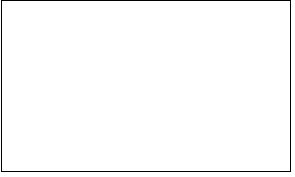
\includegraphics{figs/grabs.pdf}
%\end{graphicalabstract}

\begin{highlights}
\item Research highlights item 1
\item Research highlights item 2
\item Research highlights item 3
\end{highlights}

\begin{keywords}
automotive multiplate clutch \sep contact mechanics \sep stochastic mechanics
\end{keywords}


\maketitle

\section{Introduction}
Cost savings in automotive industry, consequences from production deficiencies, vibration phenomena elimination. Different vibration phenomena lead to increased costs. Criterion at end of line testing with clear thrash limits. Avoid driver complaints. \\
Vibration/acoustic problems due to follower loads of the sliding contact can originate e.g. from the wobbling Eigenmode \cite{fidlin2011minimal,wickramarachi2005analysis}, clutch-gear-interaction \cite{jehle2018nonlinear}, elasticity of the contact surface \cite{hetzler2009moving,jehle2016flexible}. Here: the low-frequency torsional vibration problem adressed, also called judder \cite{klement2011Fahrzeug}.\\
Three types of judder can be distinguished, namely, friction induced, pressure induced, geometrically induced \cite{drexl1990clutch}. All have in common: in sliding phase (launch, shift). It lead to torsional vibrations at low frequency which can be critical regarding drivetrain resonance and be felt by driver. 
Friction induced: sliding friction coefficient's speed dependency \cite{hinrichs1997reibungsschwingungen,kauderer1958nichtlineare}, negative gradient, negative contribution to damping. This is an instability. Pressure induced: whenever actuation piston vibrates axially, it modifies the torque, thus, torsional vibrations. External excitation. 
Geometric excitation: geometrical deviations of the sliding surfaces modulate the local normal pressure, then local frictional torque is modified. In this paper adressed. Nature of the problem: external excitation, and it is impossible to extinct it. Only reduce.(surfaces never flat because of production). The less surface deviations and the better the material homogenity (i.e., high production quality), the less vibration excitation. \\
Frequency: integer slip multiples. At clutch close, any Eigenmode can be excited because the excitation is at slip multiples and base frequency decays toward zero. Therefore critical. Here: considerations about how to obtain low judder values. This is an optimization problem \cite{albers1998Rupfen,dresig2014schwingungen,hausner2012Judder} which can only be tackled by arranging the production deficiancies in an appropriate manner. \\
Measurement difficulty with plate clutch: very bad reproducibility. Probable reason: many contacts, many uncertainties. Many measurements necessary for profound understanding of influence parameters. Therefore a non-trivial question for experimental investigations \cite{ingram2010Clutch} \\
In this contribution, a simulation which reproduces measurement quality (reproducibility, parameter influences, some dependencies). Then Monte-Carlo simulation and evaluation. 
\begin{figure}
	\centering
	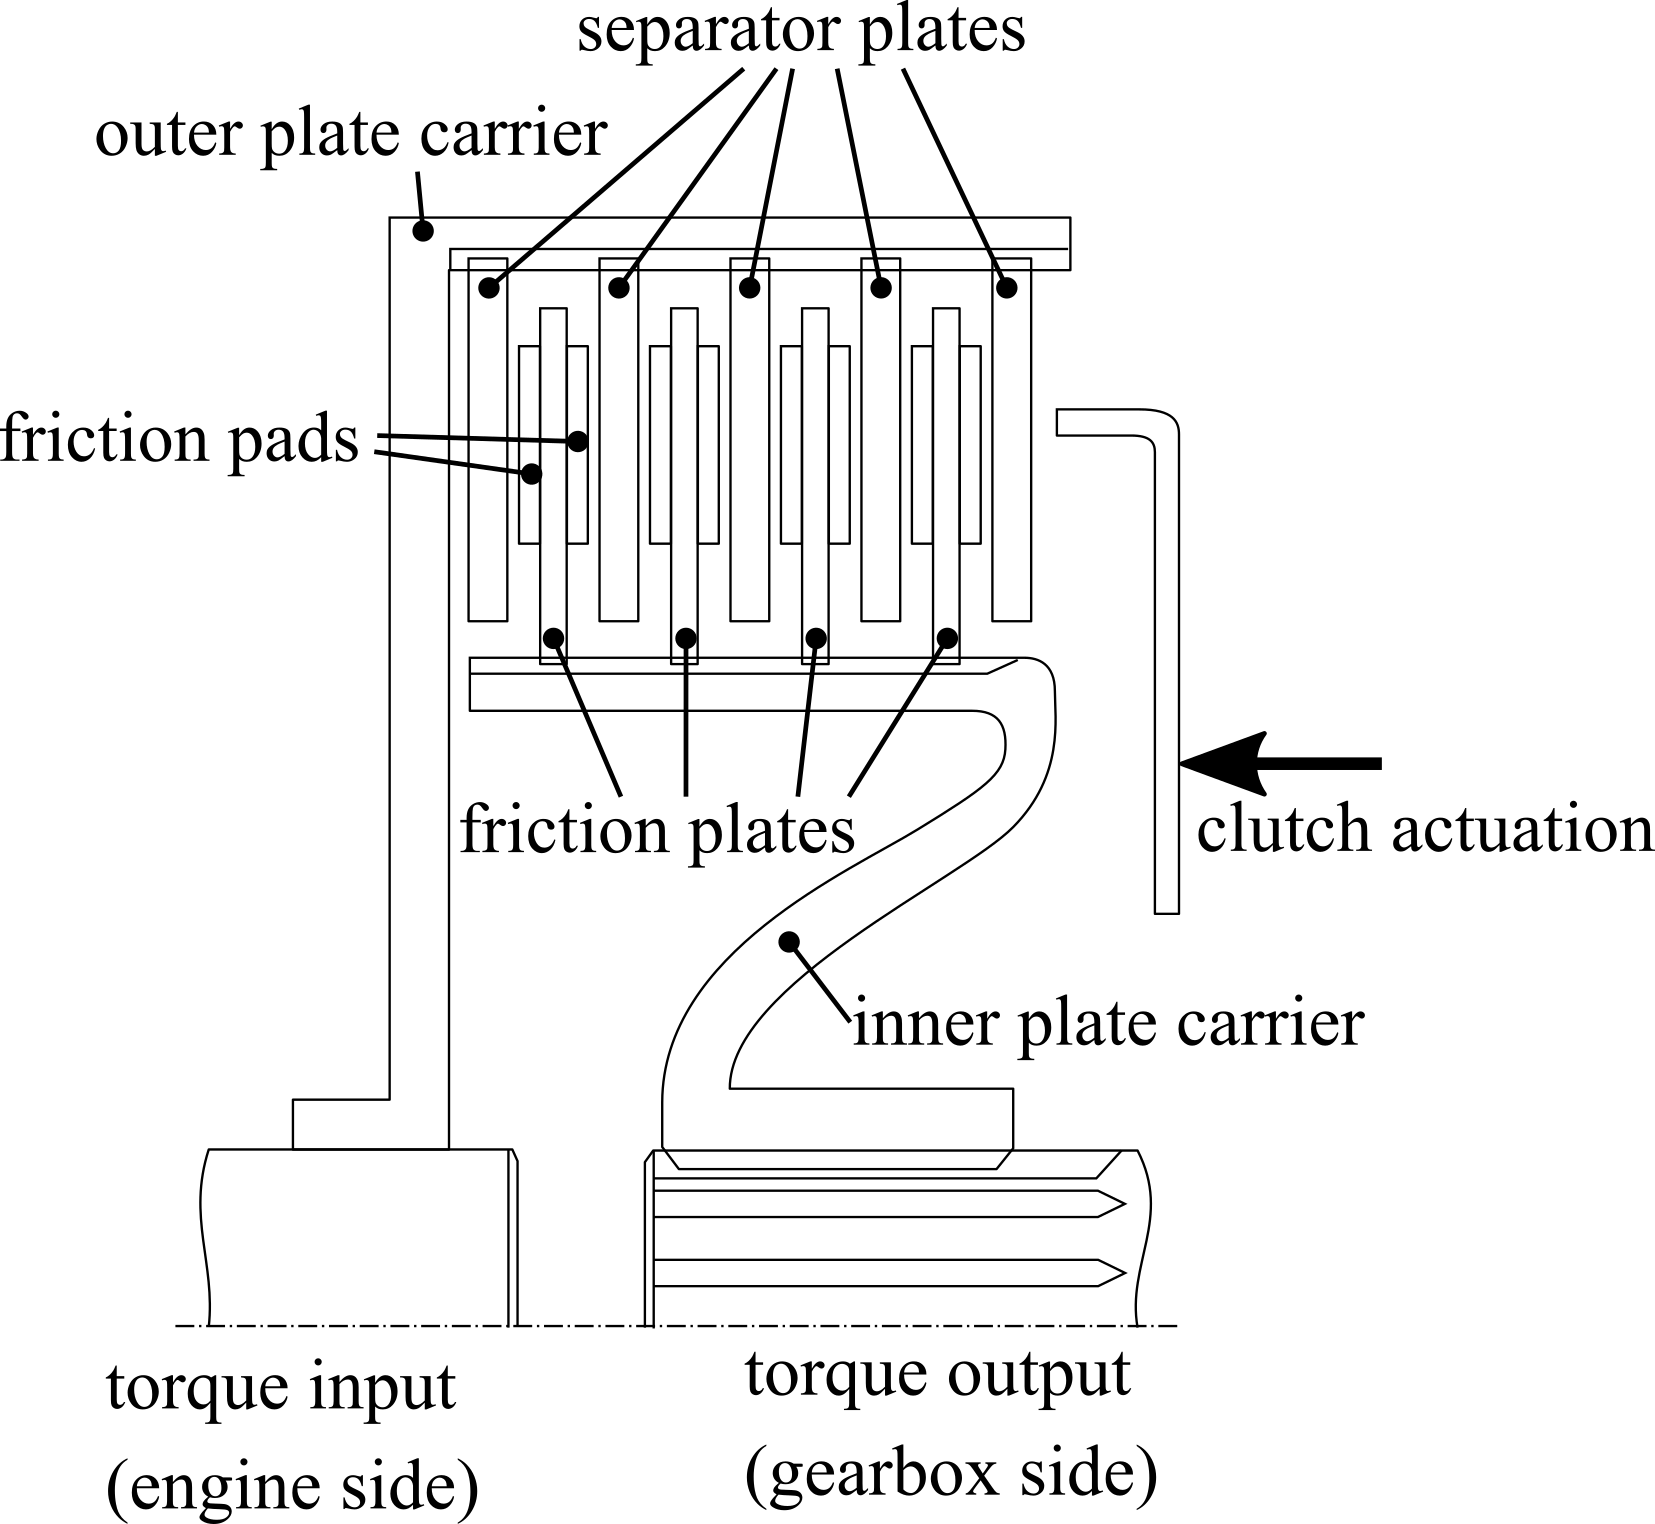
\includegraphics[scale=.75]{figs/Design.png}
	\caption{Design elements of plate clutch. }
	\label{fig:design}
\end{figure}\\
\cite{centea2001non,gregori2014Judder,jacobsson2003Aspects,jahagirdar2007Judder}. 

\section{Multiplate clutch system description}
\subsection{Design}
Multiplate clutch can be situated in a transmission, separator, ... . The design regarding judder has a uniform description: components of a multiplate clutch are friction plates, separator plates, piston, outer plate carrier (OPC) and inner plate carrier (IPC). (Fig. \ref{fig:design}). Plate carriers are connected with torque input (engine) and ouput (gearset, ...), rotate about an inertial-fixed axis. Plates mounted by spline on plate carriers, can move axially and have slight play due to clearance (Fig. \ref{fig:teeth}). Contact pads on friction plates for defined contact area; pad geometry is the secret of the plate manufacturer. Piston pushes plates in axial direction, which leads to torque transmission. \\
\subsection{Flank contact description}
There are $n_o$ and $n_i$ tooth contacts. Contact kinematics as in textbooks \cite{willner2013kontinuums}, applied for the rigid tooth geometry. 
Equal distribution. Implementation: point-plane contact. 
starting from body-fixed center, the coordinate is
\begin{align}
	& \boldsymbol{r}_f^{\mathcal{I}} = r_{pitch} \boldsymbol{e}_r^{\mathcal{B}} \left(\varphi_{left}\right) \\
	& \boldsymbol{e}_{n,f}^{\mathcal{B}} = R r\\
	& \boldsymbol{v}_f^{\mathcal{B}}  = \boldsymbol{v}_s ^{\mathcal{I}} + \boldsymbol{\omega}^{\mathcal{B}}\times \boldsymbol{r}_f\\
	& \boldsymbol{v}_{T,f}^{\mathcal{B}} = \boldsymbol{v}_f ^{\mathcal{I}}- \left(\boldsymbol{v}_f ^{\mathcal{I}}\cdot \boldsymbol{e}_{n,f}^{\mathcal{B}} \right)\boldsymbol{e}_{n,f}^{\mathcal{B}}
\end{align}
gap function \cite{willner2013kontinuums}
\begin{align}
	& g = \left(\boldsymbol{r}_f^{\mathcal{I}}-\boldsymbol{r}_f^{\mathcal{I}}\right)\cdot \boldsymbol{e}_{n,f}^{\mathcal{B}}\\
	& \dot g = \left(\boldsymbol{v}_f^{\mathcal{I}}-\boldsymbol{v}_f^{\mathcal{I}}\right)\cdot \boldsymbol{e}_{n,f}^{\mathcal{B}}
\end{align}
\begin{figure}
	\centering
	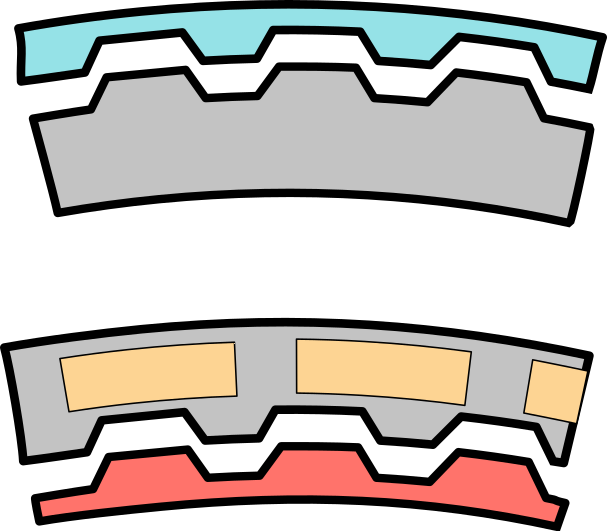
\includegraphics[scale=.75]{figs/toothcontacts.png}
	\caption{tooth contact geometry.}
	\label{fig:teeth}
\end{figure}\\
local normal force and friction force (regularized \cite{vielsack1996regularisierung}) 
\begin{align}
	& \boldsymbol{f}_n = \left\{
	\begin{array}{ll}
	(c g + d \dot g)\boldsymbol{e}_n & c g + d \dot g \leq 0\\
	0 & \textrm{else}
	\end{array}\right.\\
	& \boldsymbol{f}_t = \mu |f_n | reg(v_t) \boldsymbol{e}_t
\end{align}
with $reg(\cdot)$ the regularization of $sign(\cdot)$. The piecewise definition of the normal force represents the gap. These force act on the plate COM: 
\begin{align}
	& f = \sum f_n + f_t\\
	& t = \sum r_{f,i}\times \left(f_n + f_t\right)
\end{align}
\subsection{Pad contact description}
surface parametrization: contact ring with circular thickness distribution. Assumption: no ''waviness'', i.e., height profile symmetric on both contact sides
\begin{align}
	& \boldsymbol{r}_i = r\boldsymbol{e}_r + h\boldsymbol{e}_z\\
	& h = h_0 + \sum_{k=11}^{n}h_k \cos\left(k\varphi-\beta_k\right) 
\end{align}
Because of the periodicity, the surface can be approximated by a Fourier series, which is generated out of geometric measurements, has the advantage of an analytic formula for the surface parametrization. 
\begin{figure}
	\centering
	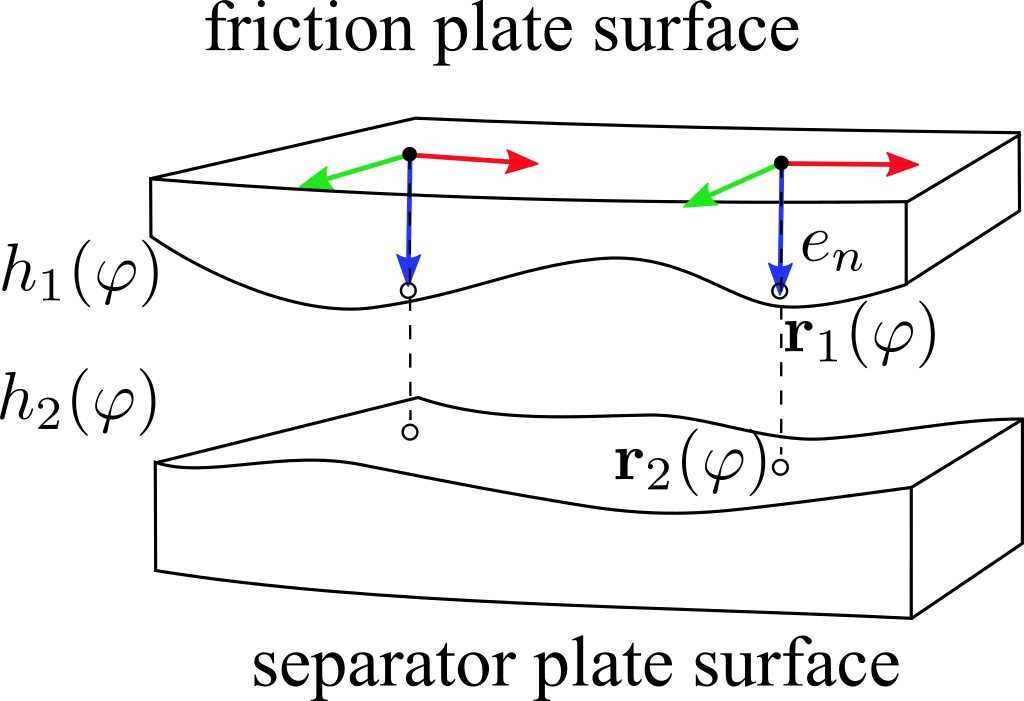
\includegraphics[scale=.75]{figs/roughsurf.png}
	\caption{Rough surface contact kinematics (simplified). }
	\label{fig:roughsurf}
\end{figure}\\
gap function \cite{willner2013kontinuums} at angle $\varphi$ and normal velocity
\begin{align}
	& g(\varphi) = \left(\boldsymbol{r}_2-\boldsymbol{r}_1\right)\cdot \boldsymbol{e}_n\\
	& \dot g(\varphi) = \left(\boldsymbol{v}_2-\boldsymbol{v}_1\right)\cdot \boldsymbol{e}_n	
\end{align}
projection on analytical formula ensures that there is no rattling effect due to mesh change. distributed friction forces: regularized, no tensile forces 
\begin{align}
&\boldsymbol{f}_{N} = f_n(g) \boldsymbol{e}_n\approx c_n g\boldsymbol{e}_n\\
&\boldsymbol{f}_{T} = \mu |\boldsymbol f_N| \boldsymbol{e}_t
\end{align}
There is no need for transition modeling between slide and stick, as only sliding states are considered in the simulation. \\
Result is the integral (sum) of all contact forces on the distributed contact. 
\begin{align}
& f = \sum f_n + f_t\\
& t = \sum r_{f,i}\times \left(f_n + f_t\right)
\end{align}
\subsection{MBS}
Finally, dynamic system equations are obtained in a MBS implementation according to the design (Figs. \ref{fig:design},\ref{fig:teeth},\ref{fig:roughsurf}). The model structure is as follows: 
4 friction plates (pad friction, tooth friction),
5 steel plates (pad friction, tooth friction), 
piston, 
opc
Piston has tilting DoF and given axial displacement 
Set of equations has the following structure 
\begin{align}
	&{M}\ddot{{q}}_{ij} + f_{ij}(q_{ij}) = 0\\
	&{M}\ddot{{q}} + f_{ij}(q) = 0
\end{align}
Boundary conditions. piston is pushed in axial direction by hydraulics. close to displacement boundary condition (elasticity of oil reservoir much higher than plates elasticity).
\section{Verification with measurements}
Clear: single simulation not reasonable. Many simulations because of spread and because many parameters can't be measured, are random. \\
stochastic influences from surface distributions are obvious. Main randomness contributors: plate mount orientation (normal distribution), initial conditions (Gaussisan distribution), friction coefficient (Gaussian distribution). In addition, material inhomogeneity, ... \\
\begin{figure}
	\centering
\begin{tikzpicture}[scale=1]
\begin{axis}[xlabel=$\varphi_{piston}$,ylabel=$T$ ,
scale = 0.43,
width=\textwidth,
xtick={0,0.5,1}, grid=major,
xticklabels={0,$\pi$,$2\pi$},
every axis y label/.style={at={(-0.2,0.5)},rotate=90}, 
every axis x label/.style={at={(0.5,-0.15)}},
%xmin=0,xmax=7,
%height = 1.0\textwidth,
%legend style={at={(0.15,0.03)},anchor=south west}, 
%legend cell align=left, 
]
\addplot[color=black,only marks,mark=*,mark size=0.6] table[x expr=\thisrowno{8}/2/pi,y expr=\thisrowno{0}] {ASCII/RandomIcMount2000.txt};
\addplot[color=red,only marks,mark=*,mark size=0.6] table[x expr=\thisrowno{8}/2/pi,y expr=\thisrowno{1}] {ASCII/RandomIcMount2000.txt};
%\legend{}
\end{axis}
\end{tikzpicture}
	\caption{measured surface distributions and harmonic interpolation.}
	\label{fig:surfdist}
\end{figure}
\begin{figure}
	\centering
	
\includegraphics[scale=.75]{figs/Fig1.pdf}
	\caption{IC influence. Time domain and frequency domain. }
	\label{fig:IC}
\end{figure}
Proof: result is a random variables. \\
\begin{figure}
\centering
\begin{tikzpicture}[scale=1]
	\begin{axis}[xlabel=$\varphi_{piston}$,ylabel=$T$ ,
	scale = 0.43,
	width=\textwidth,
	xtick={0,0.5,1}, grid=major,
	xticklabels={0,$\pi$,$2\pi$},
	every axis y label/.style={at={(-0.2,0.5)},rotate=90}, 
	every axis x label/.style={at={(0.5,-0.15)}},
	%xmin=0,xmax=7,
	%height = 1.0\textwidth,
	%legend style={at={(0.15,0.03)},anchor=south west}, 
	%legend cell align=left, 
	]
	\addplot[color=black,only marks,mark=*,mark size=0.6] table[x expr=\thisrowno{8}/2/pi,y expr=\thisrowno{0}] {ASCII/RandomIcMount2000.txt};
	\addplot[color=red,only marks,mark=*,mark size=0.6] table[x expr=\thisrowno{8}/2/pi,y expr=\thisrowno{1}] {ASCII/RandomIcMount2000.txt};
	%\legend{}
\end{axis}
\end{tikzpicture}
\caption{Matching + IC influence. Sort according to different components.}
\label{fig:matching}
\end{figure}
\begin{figure}
\centering

\includegraphics[scale=.75]{figs/Fig1.pdf}
\caption{Full parametric simulation. Parameter influences.}
\label{fig:full parametric}
\end{figure}\\

2 surface data samples. According to tests, the first part of good clutch, the second bad clutch. Reproduce this difference is part of model verification. \\

according, simulation setup: 
randomness in friction coefficient, normal stiffness, plate orientation, initial coefficients.

Stochastic 

\section{Linear regression analysis}
\section{Further regression analysis methods}

\section{Conclusion}
Boundary conditions importance: softness of actuation is important regarding intensity. \\
Friction coefficient between plates and plate carriers: stochasticity and intensity. Mainly in force model.  \\
Initial conditions: stochasticity, but not as influent as friction coefficient. \\


\section{Introduction}

The Elsevier cas-dc class is based on the
standard article class and supports almost all of the functionality of
that class. In addition, it features commands and options to format the
\begin{itemize} \item document style \item baselineskip \item front
matter \item keywords and MSC codes \item theorems, definitions and
proofs \item lables of enumerations \item citation style and labeling.
\end{itemize}

This class depends on the following packages
for its proper functioning:

\begin{enumerate}
\itemsep=0pt
\item {natbib.sty} for citation processing;
\item {geometry.sty} for margin settings;
\item {fleqn.clo} for left aligned equations;
\item {graphicx.sty} for graphics inclusion;
\item {hyperref.sty} optional packages if hyperlinking is
  required in the document;
\end{enumerate}  

All the above packages are part of any
standard \LaTeX{} installation.
Therefore, the users need not be
bothered about downloading any extra packages.

\section{Front matter}

The author names and affiliations could be formatted in two ways:
\begin{enumerate}[(1)]
\item Group the authors per affiliation.
\item Use footnotes to indicate the affiliations.
\end{enumerate}
See the front matter of this document for examples. 
You are recommended to conform your choice to the journal you 
are submitting to.

\section{Floats}
{Figures} may be included using the command,\linebreak 
\verb+\includegraphics+ in
combination with or without its several options to further control
graphic. \verb+\includegraphics+ is provided by {graphic[s,x].sty}
which is part of any standard \LaTeX{} distribution.
{graphicx.sty} is loaded by default. \LaTeX{} accepts figures in
the postscript format while pdf\LaTeX{} accepts {*.pdf},
{*.mps} (metapost), {*.jpg} and {*.png} formats. 
pdf\LaTeX{} does not accept graphic files in the postscript format. 
\begin{figure}
	\centering
		
\includegraphics[scale=.75]{figs/Fig1.pdf}
	\caption{The evanescent light - $1S$ quadrupole coupling
	($g_{1,l}$) scaled to the bulk exciton-photon coupling
	($g_{1,2}$). The size parameter $kr_{0}$ is denoted as $x$ and
	the \PMS is placed directly on the cuprous oxide sample ($\delta
	r=0$, See also Table \protect\ref{tbl1}).}
	\label{FIG:1}
\end{figure}


The \verb+table+ environment is handy for marking up tabular
material. If users want to use {multirow.sty},
{array.sty}, etc., to fine control/enhance the tables, they
are welcome to load any package of their choice and
{cas-dc.cls} will work in combination with all loaded
packages.

\begin{table}[width=.9\linewidth,cols=4,pos=h]
\caption{This is a test caption. This is a test caption. This is a test
caption. This is a test caption.}\label{tbl1}
\begin{tabular*}{\tblwidth}{@{} LLLL@{} }
\toprule
Col 1 & Col 2 & Col 3 & Col4\\
\midrule
12345 & 12345 & 123 & 12345 \\
12345 & 12345 & 123 & 12345 \\
12345 & 12345 & 123 & 12345 \\
12345 & 12345 & 123 & 12345 \\
12345 & 12345 & 123 & 12345 \\
\bottomrule
\end{tabular*}
\end{table}

\section[Theorem and ...]{Theorem and theorem like environments}

{cas-dc.cls} provides a few shortcuts to format theorems and
theorem-like environments with ease. In all commands the options that
are used with the \verb+\newtheorem+ command will work exactly in the same
manner. {cas-dc.cls} provides three commands to format theorem or
theorem-like environments: 

\begin{verbatim}
 \newtheorem{theorem}{Theorem}
 \newtheorem{lemma}[theorem]{Lemma}
 \newdefinition{rmk}{Remark}
 \newproof{pf}{Proof}
 \newproof{pot}{Proof of Theorem \ref{thm2}}
\end{verbatim}


The \verb+\newtheorem+ command formats a
theorem in \LaTeX's default style with italicized font, bold font
for theorem heading and theorem number at the right hand side of the
theorem heading.  It also optionally accepts an argument which
will be printed as an extra heading in parentheses. 

\begin{verbatim}
  \begin{theorem} 
   For system (8), consensus can be achieved with 
   $\|T_{\omega z}$ ...
     \begin{eqnarray}\label{10}
     ....
     \end{eqnarray}
  \end{theorem}
\end{verbatim}  


\newtheorem{theorem}{Theorem}

\begin{theorem}
For system (8), consensus can be achieved with 
$\|T_{\omega z}$ ...
\begin{eqnarray}\label{10}
....
\end{eqnarray}
\end{theorem}

The \verb+\newdefinition+ command is the same in
all respects as its \verb+\newtheorem+ counterpart except that
the font shape is roman instead of italic.  Both
\verb+\newdefinition+ and \verb+\newtheorem+ commands
automatically define counters for the environments defined.

The \verb+\newproof+ command defines proof environments with
upright font shape.  No counters are defined. 


\section{Bibliography}

Two bibliographic style files (\verb+*.bst+) are provided ---
{model1-num-names.bst} and {model2-names.bst} --- the first one can be
used for the numbered scheme. This can also be used for the numbered
with new options of {natbib.sty}. The second one is for the author year
scheme. When  you use model2-names.bst, the citation commands will be
like \verb+\citep+,  \verb+\citet+, \verb+\citealt+ etc. However when
you use model1-num-names.bst, you may use only \verb+\cite+ command.

\verb+thebibliography+ environment.  Each reference is a\linebreak
\verb+\bibitem+ and each \verb+\bibitem+ is identified by a label,
by which it can be cited in the text:

\noindent In connection with cross-referencing and
possible future hyperlinking it is not a good idea to collect
more that one literature item in one \verb+\bibitem+.  The
so-called Harvard or author-year style of referencing is enabled
by the \LaTeX{} package {natbib}. With this package the
literature can be cited as follows:

\begin{enumerate}[\textbullet]
\item Parenthetical: \verb+\citep{WB96}+ produces (Wettig \& Brown, 1996).
\item Textual: \verb+\citet{ESG96}+ produces Elson et al. (1996).
\item An affix and part of a reference:\break
\verb+\citep[e.g.][Ch. 2]{Gea97}+ produces (e.g. Governato et
al., 1997, Ch. 2).
\end{enumerate}

In the numbered scheme of citation, \verb+\cite{<label>}+ is used,
since \verb+\citep+ or \verb+\citet+ has no relevance in the numbered
scheme.  {natbib} package is loaded by {cas-dc} with
\verb+numbers+ as default option.  You can change this to author-year
or harvard scheme by adding option \verb+authoryear+ in the class
loading command.  If you want to use more options of the {natbib}
package, you can do so with the \verb+\biboptions+ command.  For
details of various options of the {natbib} package, please take a
look at the {natbib} documentation, which is part of any standard
\LaTeX{} installation.

\appendix
\section{My Appendix}
Appendix sections are coded under \verb+\appendix+.

\verb+\printcredits+ command is used after appendix sections to list 
author credit taxonomy contribution roles tagged using \verb+\credit+ 
in frontmatter.

\printcredits

%% Loading bibliography style file
%\bibliographystyle{model1-num-names}
\bibliographystyle{cas-model2-names}

% Loading bibliography database
%\bibliography{cas-refs}
\bibliography{Literaturliste}


%\vskip3pt

%\bio{}
%Author biography without author photo.
%Author biography. Author biography. Author biography.
%Author biography. Author biography. Author biography.
%Author biography. Author biography. Author biography.
%Author biography. Author biography. Author biography.
%Author biography. Author biography. Author biography.
%Author biography. Author biography. Author biography.
%Author biography. Author biography. Author biography.
%Author biography. Author biography. Author biography.
%Author biography. Author biography. Author biography.
%\endbio
%
%\bio{figs/pic1}
%Author biography with author photo.
%Author biography. Author biography. Author biography.
%Author biography. Author biography. Author biography.
%Author biography. Author biography. Author biography.
%Author biography. Author biography. Author biography.
%Author biography. Author biography. Author biography.
%Author biography. Author biography. Author biography.
%Author biography. Author biography. Author biography.
%Author biography. Author biography. Author biography.
%Author biography. Author biography. Author biography.
%\endbio
%
%\bio{figs/pic1}
%Author biography with author photo.
%Author biography. Author biography. Author biography.
%Author biography. Author biography. Author biography.
%Author biography. Author biography. Author biography.
%Author biography. Author biography. Author biography.
%\endbio

\end{document}

